\section{Cross Layer Analysis}

This section briefly describes the how I collect ground truth data transmission information in IP and RLC layer using QxDM in subsection 1. Subsection 2 talks about the core algorithm to enable cross layer mapping. Subsection 3 verifies the latency observations using cross layer algorithm. Subsection 4 describes about how I calculate the RLC retransmission ratio in QxDM. Subsection 5 identifies the root cause of latency by results from both emph{UDP\_{}Trace} and emph{TCP\_{}Trace}, and propose RLC \textit{Fast Re-Tx} mechanism to reduce the RLC delay.

\subsection{QxDM Tool}

% Describe what the tool does
QxDM is a real-time data collection and diagnostic logging tool for measuring mobile-based RF (Radio Frequency) performance~\cite{qxdm_flyer}. It is a Windows based monitoring application. When I perform control experiments and real application measurements, I plug in the device to the desktop or laptop with QxDM software installed. Once the experiments finishes, I filtered out the real-time monitoring information related to IP packets, RLC PDUs (protocol data unit, the smallest data transmission unit in RLC layer), and RRC states in Table~\ref{tab:QxDM.logs}, and dump the results into a log file. The 0x11EB log entry includes IP headers, IP payloads, and its customized header. Since large IP packets will be fragmented into smaller segments, the customer header could indicate the segment index of the whole IP packet. The 0x4132 and 0x4133 unveil the RLC AM (acknowledge mode) configurations, i.e. the polling function timers, the retransmission limit for a single PDU, and etc. The 0x413B, and 0x418B provides RLC PDU header and first byte payload information for both data PDUs and control PDUs (or STATUS PDUs) in both uplink and downlink directions. We wrote a QxDM log parser to aggregate the filtered entries, and apply cross layer analysis to understand the correlation between different layers. I conduct all the experiments on two devices -- Galaxy S3 with Android OS 4.1.1 and HTC One S with Android OS 4.0.4, to observe any device dependent behavior.

%QxDM provides precise RRC state information to indicate the current radio channel state. RLC data PDU and status PDU will assist us in cross layer mapping to the transport layer data, i.e. TCP/UDP. Other context information could also be found in the log, i.e. signal strength and physical layer transmission bit rate. The QxDM log is essentially a list of log entries formatted as a uniformed header with timestamp, a detailed log entry description, and a raw hex dump result.  

% Table of QxDM entries
\begin{table}
\begin{tabularx}{0.48\textwidth}{ | c | X | }
	\hline
  	\textbf{QxDM Log ID} & \textbf{Description} \\
  	\hline\hline
  	0x11EB & IP data packets \\
  	\hline
  	0x4132 & WCDMA RLC downlink acknowledge mode configuration \\
  	\hline
  	0x4133 & WCDMA RLC uplink acknowledge mode configuration \\
  	\hline
  	0x413B & WCDMA RLC uplink acknowledge mode PDU \\
  	\hline
  	0x418B & WCDMA Flexible RLC downlink acknowledge mode PDU \\
  	\hline
  	0x4125 & WCDMA RRC states \\
  	\hline
\end{tabularx}
\caption{QxDM log entries used in cross layer analysis}
\label{tab:QxDM.logs}
\end{table}

% UDP results
\subsection{Verification Latency in QxDM}

% UDP loss behavior over different states
QxDM provides the ground truth information about RRC state, so I want to validate the delay behavior based on the inferred RRC model. To verify the packet delay in the transport layer over each RRC state, I need to know the RRC state for transport layer packets and RLC layer PDUs. Since each RRC state log is only a single log entry indicating the change of RRC state, I don't have explicit RRC state information tied to each packet and PDU. Therefore, I determine the RRC states by backtracking the most recent RRC state log, then assign as attributes to the packets and PDUs so that I could acquire RRC state information directly from the packet or PDU itself. 

Because the the promotion period for PCH and FACH differs from their initial period due to additional signaling overhead, I want to distinguish between a RRC state with and without involving transitions. Since I focus on the initial period of data transmission, the RRC state promotion is more meaningful than state demotion, which is the end of whole data transmission period. So RRC state promotion is our preliminary concern for this project. We break down the normal FACH into FACH\_{}INIT and FACH\_{}PROMOTE states. Similarly, PCH was divided into PCH\_{}INIT and PCH\_{}PROMOTE. Since the FACH promotion timer is around 2 seconds and PCH promotion state is around 0.5 seconds. I define the FACH\_{}PROMOTE state as the time slot of counting back 2 seconds from the point of promoting to DCH. For the same reason, PCH\_{}PROMOTE state describes the time slot of counting back 0.5 seconds from the point of promoting to FACH. 

From the \emph{UDP\_{}Trace}, I calculate the UDP RTT by mapping the client transmitted UDP packets to the served echoed back packets through comparing the manually injected "sequence number". If both packets have the identical "sequence number" in their first four byte payload, then the RTT for the transmitted data is the timestamp difference between the two packets. Figure~\ref{fig:udp.rtt} shows the UDP RTT broken down into different RRC state and state transitions. The average RTT at FACH\_{}INIT state is \textit{2.52 s} for HTC One S and \textit{2.08 s} for Galaxy S3, which around both around \textit{190\%} greater than each one's RTT in DCH. The average RTT for FACH\_{}PROMOTE state is \textit{1.14 s} for HTC One S and \textit{1.05 s} for Galaxy S3, which are around \textit{40\%} greater than those in DCH. The result could validate the abnormal delay behavior especially during the initial part of the FACH state, namely the FACH\_{}INIT state. We could also observe a tremendous latency over PCH\_{}PROMOTE state. Because packets cannot stay in PCH during the transmission, the promotion to FACH and DCH will double the signaling overhead, which introduces more latency.

% UDP delay
% RLC Loss ratio per RRC state
\begin{figure}
\centering
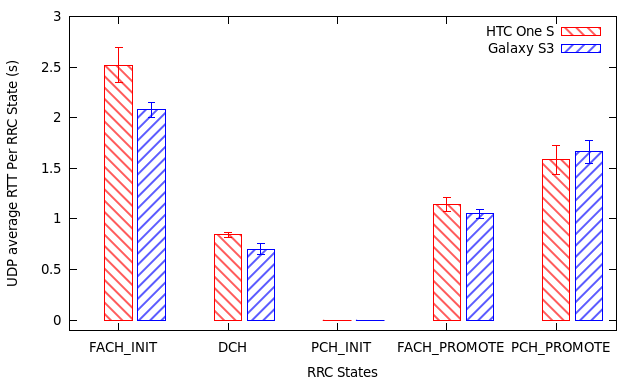
\includegraphics[width=0.45\textwidth]{figs/udp_rtt.png}
\caption{UDP RTT calculated from the QxDM log result}
\label{fig:udp.rtt}
\end{figure}

\subsection{Cross Layer Algorithm}

% Describe the mapping algorithm I use for cross-layer analysis
QxDM tool provides fine grained lower layer RLC layer transmission information. If I could correlate the transport layer packets with the RLC layer transmitted PDUs, I will have a transparent view of the link layer behaviors, especially the RLC retransmission. One of the fundamental limitation of QxDM is the partial logging issue. For example, only the header and first byte data payload will be logged for each RLC PDU. It is also possible that a small fraction of RLC PDUs cannot be captured, which lead to a unnecessary sequence number gap. Our mapping algorithm will handle all the limitations I have mentioned.

% The mapping algorithm here
The cross layer mapping algorithm is essentially a map between the complete IP packets (known as SDU) and corresponding fragmented RLC payload data bytes (known as PDU). Due to the partial logged information in QxDM, only the first data byte is captured in the log. Thus, I have to skip over the rest of the PDU, and try to match for the first data byte in the next PDU. The problem at this point is to determine the end of IP packets while I iterate through the consecutive RLC PDUs. Since each PDU could either contain the payload data dedicated to a single SDU or belongs to two SDUs. If the reminder size of the SDU cannot fulfill the largest size of PDU, then RLC protocol will concatenate the part of the next SDU to fill the rest of space~\cite{spec-3G-RLC}. Ultimately, if the accumulative mapped index equals the size of SDU, I claim to find a mapping successfully; otherwise no mapping discovered. Algorithm~\ref{alg:cross.mapping} states the detailed information of the mapping mechanism.

% the corner case of the mapping algorithm
There is a corner case in the mapping algorithm such that the QxDM cannot capture the some of the SDUs. Similar to TCP protocol, the sequence number in RLC PDUs could uniquely distinguish between every PDUs. If there are some missed PDUs, then I cannot map the first byte data for every PDU size. In that case, I could even skip over the missed PDUs and add up multiple of PDU size to hunt for a match, which is represented as "factor" variable in the mapping algorithm. However, the aggressive leap mapping mechanism cannot fully recover the corner case, especially when the missed PDUs were either the beginning or the end part of the mapped RLC list. I evaluate the improved mapping algorithm by checking the percentage of mapped IP packets in all the traces of control experiments, and the average mapping ratio is \textit{99.8\%}.

% algorithm detail
\begin{algorithm}
\begin{algorithmic}
\STATE {\textit{\textbf{Function} isCrossLayerMapped(SDU, PDU\_{}list):}}
\STATE {\textit{PDU\_{}index} = $0$}
\STATE {\textit{SDU\_{}byte\_{}index} = $0$}
\WHILE {\textit{SDU\_{}byte\_{}index} $<$ size of \textit{SDU}}
\IF {\textit{SDU[SDU\_{}byte\_{}index]} == \textit{cur\_{}PDU}}
	\STATE {\textit{cur\_{}PDU} = \textit{PDU\_{}list[PDU\_{}index]}}
	\STATE {$factor$ = \textit{cur\_{}PDU}.sn - \textit{last\_{}PDU}.sn  // sn is sequence number}
	\STATE {\textit{last\_{}PDU} = \textit{cur\_{}PDU}}
	\IF {\textit{cur\_{}PDU} has LI field in header}
		\STATE {Increase \textit{SDU\_{}byte\_{}index} by the value of LI field}
	\ELSE
    		\STATE {Increase \textit{SDU\_{}byte\_{}index} by the size of \textit{cur\_{}PDU} multiples $factor$}
    	\ENDIF
    	\IF {\textit{cur\_{}PDU}'s HE field is $2$}
    		\STATE {Break}
    \ENDIF
    	\STATE {Increase \textit{PDU\_{}index} by $1$}
\ELSE
	\STATE {Break}
\ENDIF
\ENDWHILE
\IF {\textit{SDU\_{}byte\_{}index}== size of \textit{SDU}}
	\RETURN \TRUE
\ELSE
	\RETURN \FALSE
\ENDIF
\end{algorithmic}
\caption{Decide whether one TCP/UDP packet maps to all corresponding RLC PDUs}
\label{alg:cross.mapping}
\end{algorithm}

\subsection{RLC Retransmission Calculation}

The RLC layer retransmission is a protection mechanism that maximize the reliability over a loss data transmission channel. However, it also causes the delays due to duplicate transmissions without noticing the upper layers. To assist further identifying the root cause of the latency, we first introduce how we calculate the RLC retransmission from the QxDM logs.

% how to calculate the RLC retransmission
The sequence number of the RLC PDU will uniquely identify each RLC packet. Therefore, I determine the RLC retransmission based on the duplicate of sequence numbers. Since the size of RLC PDU is only 42 bytes and is very limited, if the RLC keeps an effective throughput, it has to reduce the number of bits in the header to hold the sequence number. Therefore, the sequence number only consumes 12 bits (range of 0-4095) in the current RLC protocol~\cite{spec-3G-RLC}. As a result, sequence number is circularly reused every 4096 PDUs, and it is always increasing. To avoid over-count the duplicate sequence number in different cycle, I hard set a smaller window size of 512 to count the reappearing sequence number within that range. I determine the RRC state for each RLC PDU by backtracking to most recent RRC state log entry, and fetch the RRC state based on that log content. I break down RLC retransmitted PDUs based on their RRC states, and I calculate the retransmission ratio through dividing total number of retransmitted PDUs per RRC state by the total number of PDUs in that RRC state. 

\subsection{Root Cause Analysis and Solutions}

% explain why I want to calculate RLC layer retransmission and how to calculate
There are two possible behaviors of RLC retransmission that leads to transport layer delay. The first one is that retransmission is necessary because of noisy channel during FACH state. Based on \emph{UDP\_{}Trace}, I could see a strong correlation between RLC retransmission ratio and FACH state as an evidence. One possible solution is that application could batch the data transmission to reduce the RRC state promotion frequency~\cite{3g_rrc}. The second one is the retransmission get unnecessary delayed caused by the lagging response to the PDU loss signal. I observe it from \emph{TCP\_{}Trace} when I studied the relationship between TCP retransmission and RLC retransmission. I will also provide a improved RLC mechanism to avoid the unnecessary delay later.

% UDP trace analysis
Analyzing the \emph{UDP\_{}Trace} based on the RLC retransmission calculation methodology, we calculate the RLC retransmission ratio per RRC state in Figure~\ref{fig:RLC.Loss.Per.RRC.UDPTrace}. As we can see, the RLC retransmission among FACH and FACH\_{}PROMOTE in total are \textit{53.46\%} for HTC One S device with standard deviation of \textit{4.58\%}, and \textit{13.74\%} for Galaxy S3 devices with standard deviation of \textit{1.14\%}. It strongly suggested the significant delay over the FACH\_{}INIT and FACH\_{}PROMOTE states, which indicates the higher chance of RLC retransmission in a resource shared and noisy channel during FACH state. We could also observe that the HTC device has a higher loss rate than that of Galaxy S3. One possible explanation for device dependent behavior is that the difference in hardware module. The HTC One S was produced over Snapdragon S3 MSM8260, while the Galaxy S3 contains Snapdragon S4 MSM8960, which is the next generation of the one for HTC One S. The wireless radio techniques for Snapdragon S4 has support for larger range of network types~\cite{snapdragon}. The detailed discussion about the hardware differences is out of the scope of this paper.

% RLC Loss ratio per RRC state
\begin{figure}
\centering
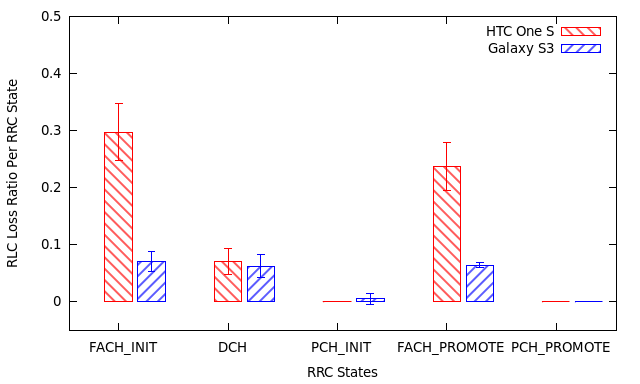
\includegraphics[width=0.45\textwidth]{figs/rlc_retx_udp.png}
\caption{Significant RLC retransmission ratio over stable FACH state and FACH promotion state strongly implies the upper layer latency during the beginning part of the data transmission}
\label{fig:RLC.Loss.Per.RRC.UDPTrace}
\end{figure}

%TCP Trace Analysis
TCP retransmission timeout (RTO) could cause apparent round trip delay due to congestion window drop by half and restarting the data transmission from the slow start phase~\cite{tcp.rto}. From the \emph{TCP\_{}Trace}, I correlate the TCP retransmission behavior with the RLC retransmission through our mapping algorithm. By capturing the root cause of the TCP RTO, I found that current RLC protocol has a sluggish response to the PDU lost signals -- the duplicate ACKs, in Figure~\ref{fig:RLC.Dup.Ack}. The delayed RLC retransmission PDUs leads TCP RTO, which further introduces latency in the transport layer. In 3GPP RLC specification, the sender only retransmits the PDU once it receives the STATUS LIST (or non-acknowledged) control PDU from the receiver, but ignores to duplicate ACKs, which is a strong hint for PDU loss~\cite{spec-3G-RLC}. If we could bring the group of retransmitted RLC PDUs from 2.8 s to 0.5 s, then we could avoid TCP RTO, reducing the latency more than 2.3 s. Therefore, I propose a RLC \textit{Fast Re-Tx} mechanism, which will retransmit the unacknowledged PDUs once the sender receives three duplicate RLC PDU ACKs. The faster reaction to loss signals could reduce RLC layer latency and further reduce the latency in transport layer.

% explain the root cause of the longer delay analysis
\begin{figure}
\centering
% DON'T add file extension for .eps images
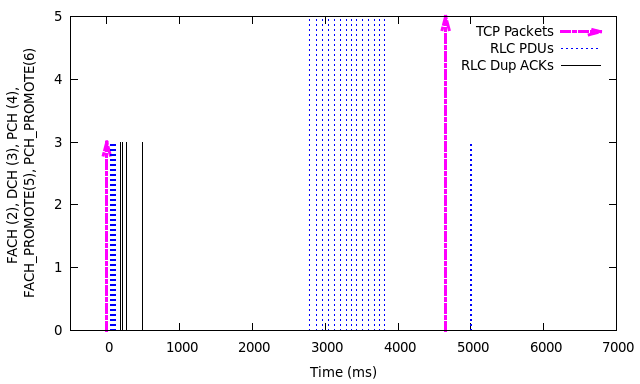
\includegraphics[width=0.45\textwidth]{figs/rlc_dup_ack.png}
\caption{Two Latency Causes: short DCH demotion timer and lagging response to the PDU lost signal}
\label{fig:RLC.Dup.Ack}
\end{figure}

\label{sec:crossAnalysis}


